\documentclass[a4paper,12pt]{article}
\usepackage{cmap}
\usepackage[T2A]{fontenc}
\usepackage[utf8]{inputenc}
\usepackage[english,russian]{babel}
\usepackage{listings}
\usepackage{amsmath}
\usepackage{amsfonts}
\usepackage{float}
\usepackage{csquotes}
\usepackage{graphicx}
\usepackage{hyphenat}
\usepackage{xcolor}
\usepackage{hyperref}
\usepackage{mathtools}
\usepackage{upgreek}


\renewcommand{\theequation}{\thesection.\arabic{equation}}


\author{Шерепа Никита}
\title{ThinkDSP. Лабораторная 8. Фильтрация и свертка.}
\date{\today}

\graphicspath{{res/screenshots}}

\begin{document}%
	
	\maketitle
	
	\newpage \tableofcontents
	\newpage \listoffigures
	\newpage \lstlistoflistings
	
	\newpage
	
	\definecolor{dkgreen}{rgb}{0,0.6,0}
	\definecolor{gray}{rgb}{0.5,0.5,0.5}
	\definecolor{mauve}{rgb}{0.58,0,0.82}
	
	\lstset{
		language=Python,                 % выбор ЯП для подсветки 
		basicstyle=\small\sffamily, % размер и начертание шрифта для подсветки кода
		numbers=left,               % где поставить нумерацию строк (слева\справа)
		numberstyle=\tiny,           % размер шрифта для номеров строк
		stepnumber=1,                   % размер шага между двумя номерами строк
		numbersep=5pt,                % как далеко отстоят номера строк от подсвечиваемого кода
		aboveskip=3mm,
		belowskip=3mm,
		showstringspaces=false,
		columns=flexible,
		captionpos=b, 
		basicstyle={\small\ttfamily},
		numbers=left,
		numberstyle=\tiny\color{gray},
		keywordstyle=\color{blue},
		commentstyle=\color{mauve},
		stringstyle=\color{dkgreen},
		breaklines=true,
		breakatwhitespace=true,
		tabsize=3
	}

	\section{Упражнение 8.1}
	
	\begin{enumerate}
		
		\item{Задание}
		
		Что случится, если при увеличении ширины гауссова окна \texttt{std} не увеличивать число элементов в окне \texttt{M}?
		
		\item{Ход работы}
		
		При увеличении ширины гауссова окна \texttt{std} без увеличения числа элементов в окне \texttt{M} прямоугольное окно превращается в "скачкообразное"
		
		\begin{figure}[H]
			\centering
			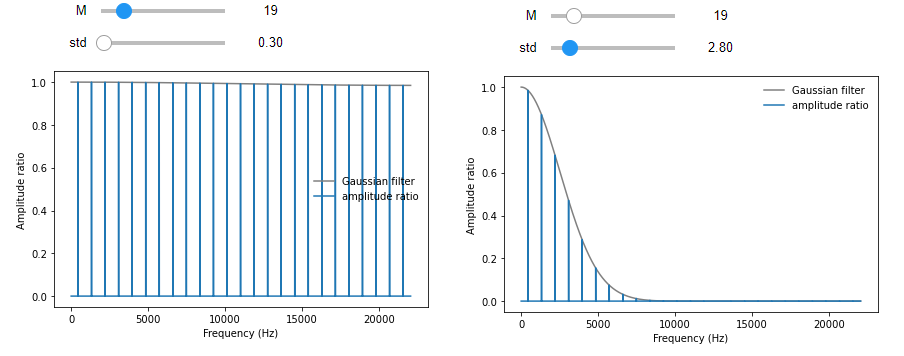
\includegraphics[width=0.75\textwidth]{1_1.png}
			\caption{1}
			\label{fig:1.1}
		\end{figure}
		\begin{figure}[H]
			\centering
			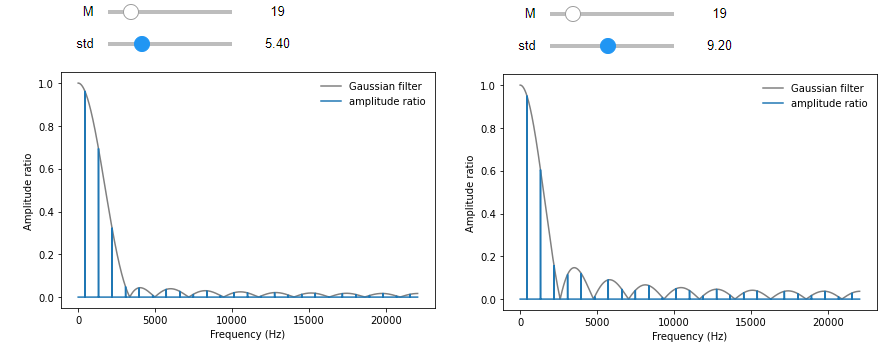
\includegraphics[width=0.75\textwidth]{1_2.png}
			\caption{2}
			\label{fig:1.2}
		\end{figure}
		\begin{figure}[H]
			\centering
			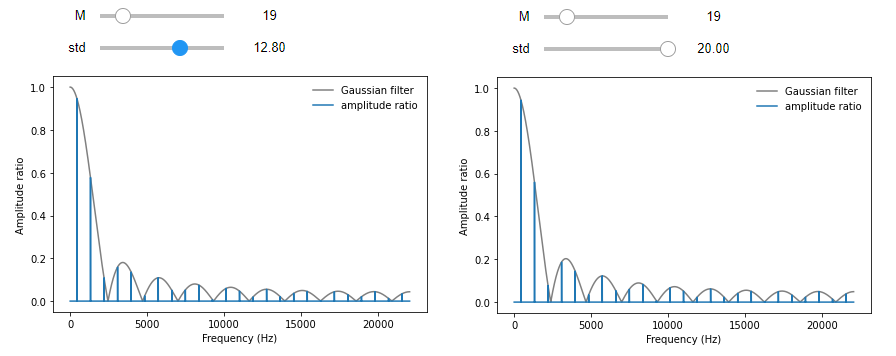
\includegraphics[width=0.75\textwidth]{1_3.png}
			\caption{3}
			\label{fig:1.3}
		\end{figure}
		
	\end{enumerate}

	\section{Упражнение 8.2}

	\begin{enumerate}
		
		\item{Задание}
		
		Преобразование Фурье гауссовой кривой - также гауссовая кривая. Для дискретного преобразования Фурье это соотношение приблизительно верно.
		
		Попробуйте его на нескольких примерах. что происходит с преобразованием Фурье, если меняется \texttt{std}
		
		\item{Ход работы}
		
		Рассмотрим Гауссиан
		
		\begin{lstlisting}[caption=Построение Гауссиана]
			import scipy.signal
			
			gaussian = scipy.signal.gaussian(M=32, std=2)
			gaussian /= sum(gaussian)
			plt.plot(gaussian)
			decorate(xlabel='Index')
		\end{lstlisting}
		\begin{figure}[H]
			\centering
			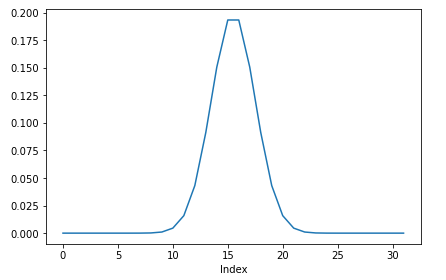
\includegraphics[width=0.75\textwidth]{2_1.png}
			\caption{Гауссиан}
			\label{fig:2.1}
		\end{figure}
		
		Применим к нему БПФ
		\begin{lstlisting}[caption=Построение Гауссиана]
			fft_gaussian = np.fft.fft(gaussian)
			plt.plot(abs(fft_gaussian))
			decorate(xlabel='Frequency (Hz)', ylabel='Amplitude')
		\end{lstlisting}
		\begin{figure}[H]
			\centering
			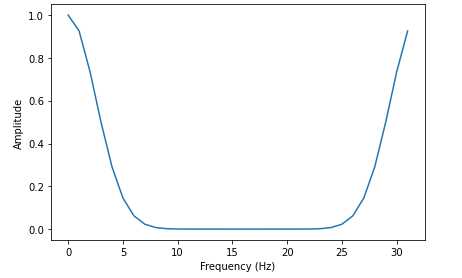
\includegraphics[width=0.75\textwidth]{2_2.png}
			\caption{Гауссиан после БПФ}
			\label{fig:2.2}
		\end{figure}
		
		Если повернуть отрицательные частоты влево, то можно четче увидеть, что это Гауссиан.
		\begin{lstlisting}[caption=Построение Гауссиана]
			N = len(gaussian)
			fft_rolled = np.roll(fft_gaussian, N//2)
			plt.plot(abs(fft_rolled))
			decorate(xlabel='Frequency (Hz)', ylabel='Amplitude')
		\end{lstlisting}
		\begin{figure}[H]
			\centering
			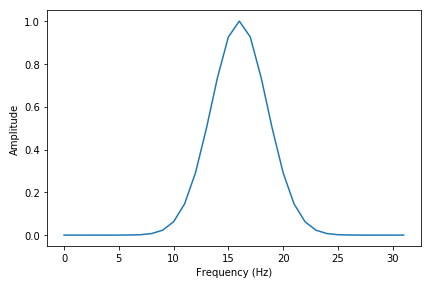
\includegraphics[width=0.75\textwidth]{2_3.png}
			\caption{Гауссиан четче}
			\label{fig:2.3}
		\end{figure}
		
		Рассмотрим функцию, которая отображает Гауссиан и БПФ Гауссиан для сравнения
		\begin{lstlisting}[caption=Функция \texttt{plot\_gaussian()}]
			def plot_gaussian(std):
			M = 32
			gaussian = scipy.signal.gaussian(M=M, std=std)
			gaussian /= sum(gaussian)
			
			plt.subplot(1, 2, 1)
			plt.plot(gaussian)
			decorate(xlabel='Time')
			
			fft_gaussian = np.fft.fft(gaussian)
			fft_rolled = np.roll(fft_gaussian, M//2)
			
			plt.subplot(1, 2, 2)
			plt.plot(np.abs(fft_rolled))
			decorate(xlabel='Frequency')
			plt.show()
			
			plot_gaussian(2)
		\end{lstlisting}
		\begin{figure}[H]
			\centering
			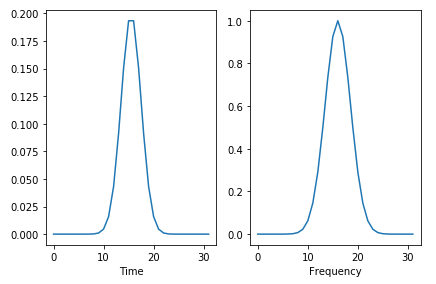
\includegraphics[width=0.75\textwidth]{2_4.png}
			\caption{Гауссиан и его БПФ}
			\label{fig:2.4}
		\end{figure}
		
		Теперь проверим, что произойдет при изменении \texttt{std}
		\begin{lstlisting}[caption=Изменяем \texttt{std}]
			from ipywidgets import interact, interactive, fixed
			import ipywidgets as widgets
			
			slider = widgets.FloatSlider(min=0.1, max=10, value=2)
			interact(plot_gaussian, std=slider);
		\end{lstlisting}
		\begin{figure}[H]
			\centering
			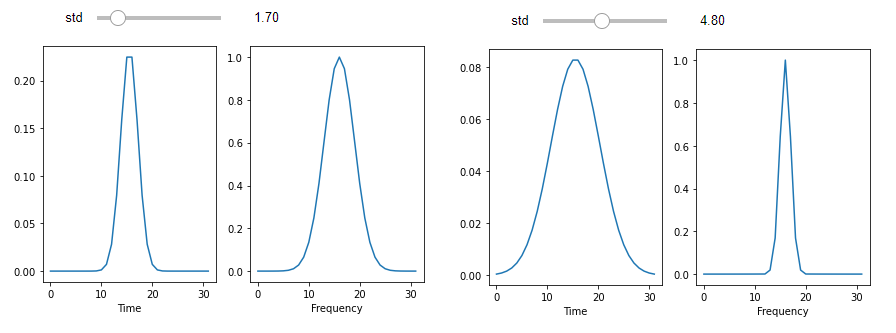
\includegraphics[width=0.75\textwidth]{2_5.png}
			\caption{Изменяем \texttt{std}}
			\label{fig:2.5}
		\end{figure}
		\begin{figure}[H]
			\centering
			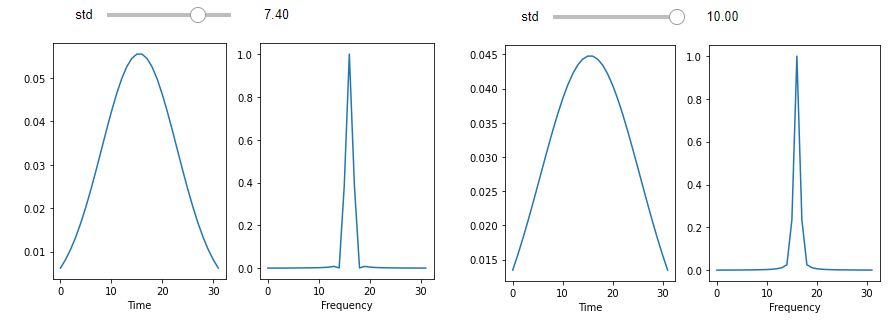
\includegraphics[width=0.75\textwidth]{2_6.png}
			\caption{Изменяем \texttt{std}}
			\label{fig:2.6}
		\end{figure}
		
		Видим, что по мере увеличения \texttt{std} Гауссиан становится шире, а его БПФ сужается.
		
		Если $f(x) = e^{-a x^2}$, что является Гауссианом со средним значением =  0 и стандартным отклонением = $1/a$, то тогда преобразование Фурье имеет вид
		
		$F(k) = \sqrt{\frac{\pi}{a}} e^{-\pi^2 k^2/a}$
		
		что является Гауссианом со стандартным отклонением = $a / \pi^2$. Таким образом, существует обратная зависимость между стандартными отклонениями $f$ и $F$.
		
		\section{Упражнение 8.3}
		
		\begin{enumerate}
			
			\item{Задание}
			
			В дополнение к Гауссовскому окну создайте окно Хемминга тех же размеров. Дополните окно нулями и напечатайте его ДПФ. Какое окно больше подходит для фильтра НЧ? Полезно напечатать ДПФ с логарифмическим масштабом \texttt{y}
			
			Поэскпериментируйте с разными окнами и размерами этих окон.
			
			\item{Ход работы}
			
			Создадим волну с частотой дискретизации = 44.1 КГц
			\begin{lstlisting}[caption=Создаем волну]
				signal = SquareSignal(freq=440)
				wave = signal.make_wave(duration=1.0, framerate=44100)
			\end{lstlisting}
			
			Теперь создадим несколько окон со стандартным отклонением Гаусса.
			\begin{lstlisting}[caption=Создаем окна]
				M = 15
				std = 2.5
				
				gaussian = scipy.signal.gaussian(M=M, std=std)   
				bartlett = np.bartlett(M)
				blackman = np.blackman(M)
				hamming = np.hamming(M)
				hanning = np.hanning(M)
				
				windows = [blackman, gaussian, hanning, hamming]
				names = ['blackman', 'gaussian', 'hanning', 'hamming']
				
				for window in windows:
					window /= sum(window)
				
				for window, name in zip(windows, names):
					plt.plot(window, label=name)
				
				decorate(xlabel='Index')
			\end{lstlisting}
			\begin{figure}[H]
				\centering
				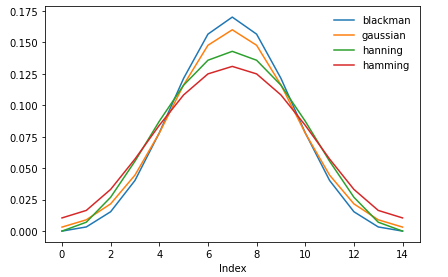
\includegraphics[width=0.75\textwidth]{3_1.png}
				\caption{Окна}
				\label{fig:3.1}
			\end{figure}
			
			Видим, что все окна похожи друг на друга. Теперь применим ДПФ
			\begin{lstlisting}[caption=Применяем ДПФ]
				def zero_pad(array, n):
				res = np.zeros(n)
				res[:len(array)] = array
				return res
				
				def plot_window_dfts(windows, names):
				for window, name in zip(windows, names):
				padded =  zero_pad(window, len(wave))
				dft_window = np.fft.rfft(padded)
				plt.plot(abs(dft_window), label=name)
				
				plot_window_dfts(windows, names)
				decorate(xlabel='Frequency (Hz)')
			\end{lstlisting}
			\begin{figure}[H]
				\centering
				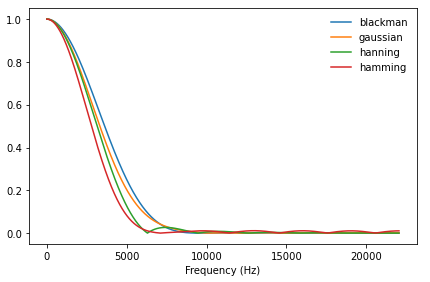
\includegraphics[width=0.75\textwidth]{3_2.png}
				\caption{Окна после ДПФ}
				\label{fig:3.2}
			\end{figure}
			Хэмминг падает быстрее всех.
			Блэкмэн падает медленней всех.
			У Хэннинга самые заметные отскоки.
			
			Теперь посмотрим на ДПФ с логарифмическим масштабом
			\begin{lstlisting}[caption=ДПФ с log-масштабом]
				plot_window_dfts(windows, names)
				decorate(xlabel='Frequency (Hz)', yscale='log')
			\end{lstlisting}
			\begin{figure}[H]
				\centering
				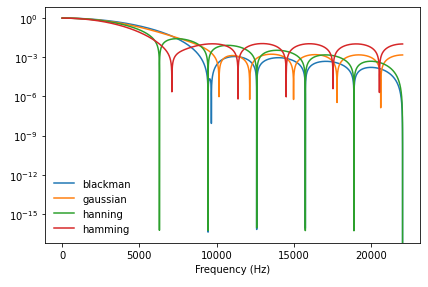
\includegraphics[width=0.75\textwidth]{3_3.png}
				\caption{ДПФ с log-масштабом}
				\label{fig:3.3}
			\end{figure}
		
			Хэмминг и Хэннинг падают быстрее остальных.
			Хэмминг и Гаусс имеют скачки.
			В итоге можно сказать, что окно Хэннинга имеет минимальные отскоки в сочетании с быстрым падением.
		
		\end{enumerate}
		
		\section{Вывод}
		
		В результате выполнения лабораторной работы получены навыки работы со свертками, построением различных окон и применения к ним ДПФ.
		
	\end{enumerate}
	
\end{document}